\documentclass[10pt,twocolumn]{article}

% ── Packages ─────────────────────────────────────────────────────────────────
\usepackage[a4paper,
            top=1.9cm, bottom=2cm,
            left=1.75cm, right=1.75cm,
            columnsep=0.58cm]{geometry}
\usepackage{graphicx}
\usepackage{booktabs}
\usepackage{caption}
\usepackage{amsmath}
\usepackage{microtype}
\usepackage{xcolor}
\usepackage{parskip}
\usepackage{natbib}
\usepackage{titlesec}
\usepackage{abstract}
\usepackage[hidelinks,colorlinks=false]{hyperref}
\usepackage{balance}   % balances final columns

% ── Typography ───────────────────────────────────────────────────────────────
\setlength{\parskip}{2pt}
\setlength{\parindent}{0pt}
\setlength{\bibsep}{2pt}

\titleformat{\section}{\normalsize\bfseries}{\thesection.}{0.4em}{}
\titleformat{\subsection}{\small\bfseries}{\thesubsection}{0.4em}{}
\titlespacing*{\section}  {0pt}{7pt}{3pt}
\titlespacing*{\subsection}{0pt}{5pt}{2pt}

\captionsetup{font=small,labelfont=bf,skip=3pt}
\renewcommand{\abstractnamefont}{\small\bfseries}
\renewcommand{\abstracttextfont}{\small}

% ── Float spacing ────────────────────────────────────────────────────────────
\setlength{\textfloatsep}{8pt plus 2pt minus 2pt}
\setlength{\floatsep}{6pt plus 2pt minus 2pt}
\setlength{\intextsep}{6pt plus 2pt minus 2pt}

% ── Title block ──────────────────────────────────────────────────────────────
\title{\large\bfseries Does Confidence-Gating Work?\\[2pt]
Empirical Evaluation of a Core AI Oversight Assumption}

\author{Rushabh Mistry\\[-1pt]
{\small Independent Researcher}\\[-2pt]
{\small \href{mailto:rushabhmistry16@gmail.com}{rushabhmistry16@gmail.com}
  \,$\cdot$\, ORCID:
  \href{https://orcid.org/0009-0001-0568-3993}{0009-0001-0568-3993}}\\[3pt]
{\small Preprint --- this version has not been peer reviewed
  \,$\cdot$\, Version 1.0, July 2026}\\[-2pt]
{\small Code and data:
  \url{https://github.com/Rushhaabhhh/confidence-gating-evaluation}}}

\date{}

% ─────────────────────────────────────────────────────────────────────────────
\begin{document}

\twocolumn[
  \maketitle\vspace{-8pt}
  \begin{onecolabstract}\small
  Three 2026 governance frameworks (Singapore's Model AI Governance Framework
  for Agentic AI, the U.S.\ NIST/NCCoE concept paper on agent identity and
  authorisation, and the EU~AI~Act, Articles~14--15) require ``meaningful
  human oversight'' of autonomous AI agents. A common implementation assumption
  is that agents can flag low-confidence decisions for human review. We test
  this assumption empirically. To our knowledge, this is among the first
  evaluations of confidence-gating measured directly against the oversight
  assumptions of these frameworks; the underlying observation that language
  models are poorly calibrated on difficult tasks is consistent with prior
  work. Verbalized confidence is elicited from two models (Llama~3.3~70B and
  Gemini~2.5~Flash) across four domains ($N{=}2{,}004$ decisions). For the
  models and benchmarks evaluated, the assumption holds on structured question
  answering: flagging the least-confident 10\% of decisions finds errors at
  $1.7$--$2.9\times$ the base rate. On an open-ended software-engineering
  judgment task (SWE-bench Verified difficulty estimation), it provides little
  to no value: lift~$\approx1.0$ for both models, and stated confidence
  occupies so narrow a band ($\sigma{<}0.06$) that fixed thresholds are
  ineffective. Post-hoc recalibration reduces aggregate calibration error by
  more than 50\% in every condition, yet does not restore per-decision
  discrimination. In a preliminary comparison on SWE-bench ($n{=}110$),
  self-consistency (three samples with majority-vote agreement) raises lift
  to~2.06, suggesting that multi-sample strategies warrant further
  investigation as oversight mechanisms for open-ended agent tasks. A
  prototype HMAC-signed audit log demonstrates the tamper-evidence requirement
  these frameworks also specify. Within this experimental scope, the
  governance implication is that confidence-gating requirements which do not
  distinguish by task type risk failing on the open-ended judgments
  characteristic of many deployed agent settings.
  \end{onecolabstract}
  \vspace{5pt}
]

% ── 1. INTRODUCTION ───────────────────────────────────────────────────────────
\section{Introduction}

Autonomous AI agents are being deployed in software engineering, finance, and
operations faster than the oversight mechanisms to govern them. Three major 2026
governance instruments independently formalise two requirements: agents must
support \emph{meaningful human oversight} and produce \emph{tamper-evident audit
trails}~\citep{imda2026,nist2026,euaiact2024}. Calls for greater visibility into
deployed agents make the same case from the research
side~\citep{chan2024}.

A natural and widely assumed implementation of the oversight requirement is
\textbf{confidence-gating}: the agent flags any decision whose stated confidence
falls below a threshold, directing limited human attention to the decisions most
likely to be wrong~\citep{galileo2026,parasuraman2010}. This assumption appears
in practitioner guides, evaluation pipelines, and proposed technical
standards for agent deployment.

What has not been measured, in the context these frameworks care about, is
whether the assumption holds. Do current models produce confidence estimates that
actually identify their errors? Do those estimates work on the \emph{kinds of
tasks} agents perform in practice, such as open-ended, multi-step judgments, or
only on structured question answering?

This paper reports such a measurement for two widely deployed models across
four benchmarks. We make three contributions:

\textbf{(1)~An empirical test of the confidence-gating assumption} across four
task types and two models, with bootstrap confidence intervals and permutation
tests. On the three structured QA domains, the assumption largely holds for the
models tested. On software-engineering difficulty judgment, it does not.

\textbf{(2)~A preliminary comparison with self-consistency} on agent-style
tasks. Where verbal confidence yields lift~$\approx1.0$ on SWE-bench,
vote-based self-consistency over three samples yields lift~$=2.06$ on the same
items ($n{=}110$).

\textbf{(3)~A prototype audit log} that implements the tamper-evidence
requirement in the Python standard library using standard cryptographic
constructions, with a field-by-field mapping to regulatory clauses.

% ── 2. WHY THIS TEST MATTERS ──────────────────────────────────────────────────
\section{Why This Test Matters}

The governance frameworks do not run experiments. The IMDA
framework~\citep{imda2026} incorporates feedback from more than 60~companies
(version~1.5, May~2026) but provides principles, not measurements. NIST's
approach is ``explicitly facilitative rather than
prescriptive''~\citep{csa2026nist}: the agency identifies gaps and co-invests
with industry but has not benchmarked specific oversight mechanisms. The
EU~AI~Act (Art.~14(4)(b)) requires systems to support awareness of automation
bias~\citep{parasuraman2010} and (Art.~14(4)(d)) to enable human override, but
specifies neither how to measure confidence nor what threshold to use.

The research community has established that LLMs are systematically
overconfident~\citep{guo2017,tian2023,xiong2024} and that verbalized confidence
is often better calibrated than token probabilities for models tuned with
human feedback~\citep{ouyang2022,tian2023,kadavath2022}. Concurrent work on
coding agents finds severe overconfidence across pre-, mid-, and post-execution
stages~\citep{kaddour2026}. Selective
prediction~\citep{geifman2017}, conformal prediction~\citep{vovk2005}, and
sampling-based uncertainty estimators~\citep{manakul2023,kuhn2023} offer richer
frameworks for assessing when a model can and cannot be trusted, and studies of
human--AI teams show that effective reliance depends on humans knowing when to
trust the model~\citep{bansal2021}. To our knowledge, however, these methods
have not been evaluated against the specific oversight requirements of the 2026
frameworks, or on the task types those frameworks target.

What has not been measured is whether confidence provides a \emph{useful
oversight trigger}: not just a calibrated number, but a number that actually
finds errors, and whether this varies by task type in ways that matter for
how governance requirements should be written.

% ── 3. REGULATORY MAPPING ─────────────────────────────────────────────────────
\section{Regulatory Requirements and Audit Record}

Table~\ref{tab:mapping} maps each field of the proposed per-decision audit
record to the specific regulatory clause it satisfies. This is the paper's
governance engineering contribution: translating three sets of prose requirements
into one concrete data structure that a compliance team could build against.

\begin{table}[t]
\centering\small
\setlength{\tabcolsep}{3.5pt}
\caption{Proposed audit-record fields and the requirements each satisfies.}
\label{tab:mapping}
\begin{tabular}{@{}p{3.0cm}p{4.7cm}@{}}
\toprule
\textbf{Field} & \textbf{Requirement} \\
\midrule
\texttt{step\_id, timestamp}    & IMDA: lifecycle monitoring \\
\texttt{agent\_id}              & NCCoE: attribute actions to
                                  non-human entity \\
\texttt{action, input\_hash}    & IMDA: record agent action and intent;
                                  hash limits data exposure \\
\texttt{confidence}             & Art.~14(4)(b): automation-bias
                                  awareness \\
\texttt{oversight\_flagged}     & Art.~14(4)(d): trigger for human
                                  override \\
\texttt{prev\_hash}             & NCCoE: tamper-evidence via chain
                                  integrity \\
\texttt{signature}              & NCCoE: non-repudiation \\
\bottomrule
\end{tabular}
\end{table}

The \texttt{confidence} and \texttt{oversight\_flagged} fields are useful only
if the confidence signal is informative. The rest of this paper tests that.

% ── 4. METHOD ─────────────────────────────────────────────────────────────────
\section{Method}

\subsection{Tasks}

We evaluate across four domains spanning qualitatively different task structures.
\textbf{SWE-bench Verified}~\citep{jimenez2024} contains genuine GitHub issues;
models estimate $p(\text{fix}{>}15\,\text{min})$ against human difficulty
labels. This is an \emph{external difficulty judgment}: the model predicts a
human annotation, not its own correctness.
\textbf{GSM8K}~\citep{cobbe2021} provides math word problems with exact numeric
answers.
\textbf{MMLU}~\citep{hendrycks2021} samples academic MCQs across 20~subjects.
\textbf{TruthfulQA}~\citep{lin2022} provides adversarial factual questions.
On the three QA domains, models assess $p(\text{own answer is correct})$, a
genuinely introspective quantity. This construct difference matters: the SWE-bench
null result may partly reflect that models are poor difficulty estimators, not
only poor introspectors.

\subsection{Models and elicitation}

Llama~3.3 70B (Groq) and Gemini~2.5 Flash (Google AI Studio) are evaluated via
public APIs; no fine-tuning is performed. Each item receives a single probability
elicitation ($0$--$100$) at temperature~$0$, with a fixed random seed (42) for
item sampling. An earlier design eliciting a binary prediction plus a
separate confidence rating led to uniformly high confidence regardless of
direction, silently disabling the oversight gate; a few-shot prompt variant was
also ablated for Llama~3.3~70B (results in the repository).

For self-consistency~\citep{wang2023sc}, the same items are queried three times
at temperature~$0.3$; the fraction voting for the majority answer serves as the
confidence estimate. This is a simplified variant of
SelfCheckGPT~\citep{manakul2023}, adapted for binary classification tasks.

\subsection{Metrics}

\textbf{Oversight lift} is the primary metric: the error rate among the
least-confident 10\% of decisions divided by the overall base error rate. Lift
$>1$ means low confidence reliably identifies errors; lift~$\approx1$ means the
gate adds no value over random selection. \textbf{AUC-RC}~\citep{geifman2017}
(area under the risk-coverage curve) measures whether sorting by confidence
ranks decisions by correctness globally. Both metrics are reported with
percentile bootstrap 95\%~CIs (2{,}000 resamples, seed~42) and permutation
$p$-values (10{,}000 permutations) for domain comparisons. The three domain
contrasts against SWE-bench are planned comparisons; we report unadjusted
$p$-values and note that all three also survive a Bonferroni correction at
$\alpha{=}0.05$ (adjusted threshold $0.0167$).

We also report ECE~\citep{guo2017} and Brier
score~\citep{brier1950,gneiting2007} before and after three post-hoc
recalibration methods (temperature scaling, Platt scaling~\citep{platt1999},
and isotonic regression~\citep{zadrozny2002}), each evaluated five-fold
out-of-sample. Confidence-in-own-answer standard deviation~$\sigma$ flags
\emph{confidence collapse} when $\sigma{<}0.10$.

% ── 5. RESULTS ────────────────────────────────────────────────────────────────
\section{Results}

\subsection{Confidence-gating works on structured QA but fails on SWE-bench}

Figure~\ref{fig:lift} shows the main result. On SWE-bench, both models produce
lift~$\approx1$: the least-confident 10\% of decisions are only marginally more
error-prone than average (Llama~1.03, Gemini~1.29). Flagging those items
provides essentially no oversight value. On GSM8K, MMLU, and TruthfulQA, lift
is substantially above~1 for the most part: 2.86, 2.06, and 2.41 for Llama;
$0.82^\dagger$, 1.91, and 1.67 for Gemini.

The domain dependence is statistically robust within this sample. The
Llama~70B GSM8K--SWE-bench lift difference is $+1.83$ (95\%~CI
$[+1.03,+2.63]$, permutation $p{<}0.001$); MMLU--SWE-bench is $+1.02$
($[+0.14,+1.90]$, $p{=}0.014$); TruthfulQA--SWE-bench is $+1.38$
($[+0.32,+2.45]$, $p{=}0.009$). All three contrasts survive Bonferroni
correction. A two-proportion $z$-test finds no significant accuracy difference
between models on SWE-bench ($\Delta{=}{-}0.008$, $p{=}0.90$), which argues
against a purely model-specific explanation.

{\small\textit{$^\dagger$Gemini's GSM8K lift of 0.82 reflects complete
confidence collapse ($\sigma{=}0.000$): every item received 100\% confidence,
so the flagged decile has no different error rate from average. This collapse
was observed under the default elicitation prompt and may be sensitive to
prompt format; it should be read as an illustrative failure mode of one
model--benchmark--prompt combination rather than a general property.}}

The reliability diagrams (Figure~\ref{fig:reliability}) confirm the calibration
picture. On GSM8K, Llama achieves 69.2\% accuracy but reports 98.6\% mean
confidence (ECE~$=0.294$). Gemini reports 100\% confidence on every item
($\sigma{=}0.000$, ECE~$=0.440$). On MMLU and TruthfulQA both models are better
calibrated.

The confidence distributions (Figure~\ref{fig:confidence}) explain why the gate
fails: $\sigma{<}0.10$ in every condition. The distributions of correct and
incorrect decisions overlap almost entirely on SWE-bench. No fixed threshold
cleanly separates them; the same cutoff flags 8.7\% of one model's decisions
and 0\% of another's, not because the models differ in reliability but because
their distributions sit at different absolute levels.

\subsection{Post-hoc calibration fixes aggregate error but not the gate}

Figure~\ref{fig:calibration} shows that post-hoc recalibration substantially
reduces ECE. Platt scaling reduces Llama's SWE-bench ECE from~0.201 to~0.015
(five-fold out-of-sample). In every condition, at least one method reduces ECE
by more than 50\% relative. Aggregate calibration is technically recoverable
without retraining~\citep{guo2017,tian2023}.

However, this does not restore the oversight gate. Post-hoc calibration corrects
the \emph{aggregate} relationship between stated confidence and empirical
accuracy, but it cannot manufacture per-decision discrimination absent from the
raw signal: the recalibration maps are monotonic, so the ranking of decisions
is unchanged. On SWE-bench, corrected confidence still does not rank decisions
by correctness because the underlying signal is uniformly high. We regard this
distinction between aggregate calibration and per-decision discrimination as
the paper's central technical point for oversight design.

\subsection{Self-consistency is a stronger signal on SWE-bench in a
preliminary comparison}

Figure~\ref{fig:sc} shows the self-consistency comparison on SWE-bench and
GSM8K (Llama~3.3 70B, $n{=}110$, 3~samples each). On SWE-bench, verbal
confidence yields lift~$=1.47$ and AUC-RC~$=0.669$; self-consistency yields
lift~$=2.06$ and AUC-RC~$=0.623$. In this preliminary comparison,
vote-fraction agreement is the substantially stronger error signal for the
open-ended task. On GSM8K, verbal confidence is
the stronger signal (lift~$=2.86$ vs.\ SC~$=1.95$), consistent with models
being able to express genuine introspective uncertainty about arithmetic.

A plausible mechanism is that sampling probes the model's implicit probability
distribution over answers, making consistency a richer signal than a verbalised
number produced in a single forward pass~\citep{manakul2023,kuhn2023}. For
governance frameworks requiring an oversight trigger on agent tasks, verbal
confidence was insufficient in our experiments; multi-sample agreement provided
a meaningfully better signal on this task at a $3\times$ API cost per decision,
which may be acceptable for high-stakes items. Given the sample size, this
result motivates further investigation rather than an immediate policy
prescription.

\subsection{Miscalibration concentrates on easy tasks}

Stratifying Llama~70B on SWE-bench by difficulty: on issues labelled
``$<$15\,min fix'' the model is 30\% accurate while reporting 81\% mean
confidence (gap~$+0.51$). On 15-min-to-4-hour issues the gap is under 0.10.
The model treats nearly all issues as hard, failing precisely where an overseer
would least expect it. By repository, overconfidence concentrates on
\texttt{sphinx-doc} (gap~$+0.31$) and \texttt{sympy} ($+0.23$).

% ── 6. AUDIT LOG ─────────────────────────────────────────────────────────────
\section{Implementing the Audit-Trail Requirement}

We implement the Table~\ref{tab:mapping} schema as an append-only,
hash-chained, HMAC-signed log using only the Python standard library. The
construction itself is standard, drawing on classic secure-logging
designs~\citep{bellareyee1997,schneierkelsey1998,crosbywallach2009}; the
contribution is the mapping to the 2026 regulatory clauses, not the
cryptography. Each entry stores
\texttt{prev\_hash} (SHA-256 of the previous entry's canonical JSON) and a
\texttt{signature} (HMAC-SHA256 over the entry content). A \texttt{verify()}
function re-walks the chain and localises the first failure.

Two insider-attack simulations are run on a 150-entry chain: flipping
\texttt{oversight\_flagged} from \texttt{true} to \texttt{false} (suppressing a
review trigger), and rewriting a \texttt{confidence} value upward (faking
certainty). Both are detected and localised to the exact tampered entry; the
intact chain verifies cleanly.

This is a prototype. HMAC is symmetric; production requires asymmetric
signatures (e.g., Ed25519) and managed key rotation. What it demonstrates
(append-chaining, per-entry signing, and tamper localisation) matches what the
NIST/NCCoE concept paper asks for at the mechanism level.

% ── 7. DISCUSSION ─────────────────────────────────────────────────────────────
\section{Discussion}

\textbf{Why confidence fails on the agent-style task.}
SWE-bench elicits $p(\text{fix}{>}15\,\text{min})$, an external difficulty
prediction against a human annotation, not a self-assessment of the model's
correctness. Even a perfectly introspective model might have no useful prior over
fix duration. The QA tasks elicit $p(\text{own answer is correct})$, a
genuinely introspective quantity. Within this evaluation, the models tested
appear capable of meaningful self-assessment on closed-ended reasoning but not
on open-ended difficulty estimation. Both failure modes are
governance-relevant; they call for different interventions.

\textbf{Implications for framework design.}
A requirement that agents ``flag low-confidence outputs'' without specifying task
type is likely to be implemented with verbal confidence gates, which worked on
the structured tasks and failed on the open-ended judgment task in our
evaluation. The specific recommendation is:
governance requirements for confidence-based oversight should (a)~specify whether
they intend introspective confidence or difficulty estimation, (b)~require
empirical validation that the chosen signal provides oversight lift~$>1$ on the
target task distribution, and (c)~consider multi-sample agreement as a candidate
alternative for open-ended tasks, pending replication at larger scale.

\textbf{Limitations.}
The study uses single-turn judgment proxies for multi-step agent behaviour;
results may not transfer to full agentic rollouts. Only two model families were
tested, and results should not be generalised beyond them; reasoning models with
chain-of-thought may have different self-assessment
properties~\citep{kadavath2022}. Findings may also be sensitive to the
elicitation prompt format, which was ablated for only one model. Sample sizes
of 110--250 per condition produce CIs spanning 0.08--0.12~ECE units. The
self-consistency comparison is preliminary ($n{=}110$, one model, SWE-bench and
GSM8K only). The audit log uses symmetric signing. Finally, the regulatory
landscape is moving: under the EU Digital Omnibus amendments agreed in 2026,
the application of the AI~Act's high-risk obligations (Annex~III) has been
deferred to December~2027, so the operative timeline for Article~14 compliance
is later than originally scheduled.

% ── 8. CONCLUSION ─────────────────────────────────────────────────────────────
\section{Conclusion}

Three 2026 governance frameworks require confidence-based human oversight of AI
agents but do not test whether the mechanism works. We report such a test for
two widely deployed models across four benchmarks. For the models and tasks
evaluated, verbalized confidence provides a useful oversight signal on
structured QA (lift up to~2.9) but not on software-engineering difficulty
judgment, an open-ended agent-style task (lift~$\approx1.0$). Post-hoc
recalibration repairs aggregate calibration but not per-decision
discrimination. A preliminary self-consistency comparison ($n{=}110$) raises
SWE-bench lift to~2.06. Within this scope, the results suggest that governance
frameworks mandating confidence-gating without specifying task type, or without
requiring empirical validation on the target distribution, risk failing
silently on the open-ended judgments where deployed agents commonly operate.

\paragraph{Data and code availability.}
All elicitation data, analysis scripts, figures, and the audit-log
implementation are available at
\url{https://github.com/Rushhaabhhh/confidence-gating-evaluation}. Experiments
use fixed seeds and temperature-0 elicitation; every number and figure in this
paper can be regenerated from the committed data without API access
(\texttt{verify\_claims.sh}).

% ── REFERENCES ────────────────────────────────────────────────────────────────
\balance
\begin{thebibliography}{31}\small\raggedright

\bibitem[Bansal et~al.(2021)]{bansal2021}
Bansal, G., Wu, T., Zhou, J., Fok, R., Nushi, B., Kamar, E., Ribeiro, M.\,T.,
\& Weld, D.\,S. (2021). Does the whole exceed its parts? The effect of AI
explanations on complementary team performance. \textit{CHI~2021}.

\bibitem[Bellare \& Yee(1997)]{bellareyee1997}
Bellare, M.\ \& Yee, B. (1997). Forward integrity for secure audit logs.
Technical report, University of California, San Diego.

\bibitem[Brier(1950)]{brier1950}
Brier, G.\,W. (1950). Verification of forecasts expressed in terms of probability.
\textit{Monthly Weather Review}, 78(1):1--3.

\bibitem[Chan et~al.(2024)]{chan2024}
Chan, A. et~al. (2024). Visibility into AI Agents. \textit{FAccT~2024},
pp.~958--973.

\bibitem[Cobbe et~al.(2021)]{cobbe2021}
Cobbe, K. et~al. (2021). Training verifiers to solve math word problems.
\textit{arXiv:2110.14168}.

\bibitem[Crosby \& Wallach(2009)]{crosbywallach2009}
Crosby, S.\,A.\ \& Wallach, D.\,S. (2009). Efficient data structures for
tamper-evident logging. \textit{USENIX Security~2009}.

\bibitem[CSA(2026)]{csa2026nist}
Cloud Security Alliance (2026). \textit{NIST AI Agent Standards Initiative}.
CSA Lab Note.

\bibitem[EU(2024)]{euaiact2024}
Regulation (EU) 2024/1689 (EU AI Act), Articles~14 and~15, as amended.

\bibitem[Galileo(2026)]{galileo2026}
Galileo (2026). \textit{How to Build Human-in-the-Loop Oversight for AI Agents}.

\bibitem[Geifman \& El-Yaniv(2017)]{geifman2017}
Geifman, Y.\ \& El-Yaniv, R. (2017). Selective classification for deep neural
networks. \textit{NeurIPS~2017}.

\bibitem[Gneiting \& Raftery(2007)]{gneiting2007}
Gneiting, T.\ \& Raftery, A.\,E. (2007). Strictly proper scoring rules,
prediction, and estimation. \textit{JASA}, 102(477):359--378.

\bibitem[Guo et~al.(2017)]{guo2017}
Guo, C., Pleiss, G., Sun, Y., \& Weinberger, K.\,Q. (2017). On calibration of
modern neural networks. \textit{ICML~2017}.

\bibitem[Hendrycks et~al.(2021)]{hendrycks2021}
Hendrycks, D. et~al. (2021). Measuring massive multitask language understanding.
\textit{ICLR~2021}.

\bibitem[IMDA(2026)]{imda2026}
Infocomm Media Development Authority, Singapore (2026). \textit{Model AI
Governance Framework for Agentic AI}, version~1.5, May~2026.

\bibitem[Jimenez et~al.(2024)]{jimenez2024}
Jimenez, C.\,E.\ et~al. (2024). SWE-bench: Can language models resolve real
GitHub issues? \textit{ICLR~2024}.

\bibitem[Kadavath et~al.(2022)]{kadavath2022}
Kadavath, S.\ et~al. (2022). Language models (mostly) know what they know.
\textit{arXiv:2207.05221}.

\bibitem[Kaddour et~al.(2026)]{kaddour2026}
Kaddour, J., Patel, S., Dovonon, G., Richter, L., Minervini, P., \& Kusner,
M.\,J. (2026). Agentic uncertainty reveals agentic overconfidence.
\textit{arXiv:2602.06948}.

\bibitem[Kuhn et~al.(2023)]{kuhn2023}
Kuhn, L., Gal, Y., \& Farquhar, S. (2023). Semantic uncertainty: linguistic
invariances for uncertainty estimation in natural language generation.
\textit{ICLR~2023}.

\bibitem[Lin et~al.(2022)]{lin2022}
Lin, S., Hilton, J., \& Evans, O. (2022). TruthfulQA: measuring how models
mimic human falsehoods. \textit{ACL~2022}.

\bibitem[Manakul et~al.(2023)]{manakul2023}
Manakul, P., Liusie, A., \& Gales, M.\,J.\,F. (2023). SelfCheckGPT:
zero-resource black-box hallucination detection for generative large language
models. \textit{EMNLP~2023}.

\bibitem[NIST/NCCoE(2026)]{nist2026}
NIST/NCCoE (2026). \textit{Accelerating the Adoption of Software and AI Agent
Identity and Authorization}. Concept paper, initial public draft,
February~2026.

\bibitem[Ouyang et~al.(2022)]{ouyang2022}
Ouyang, L. et~al. (2022). Training language models to follow instructions with
human feedback. \textit{NeurIPS~2022}.

\bibitem[Parasuraman \& Manzey(2010)]{parasuraman2010}
Parasuraman, R.\ \& Manzey, D.\,H. (2010). Complacency and bias in human use
of automation: an attentional integration. \textit{Human Factors}, 52(3):381--410.

\bibitem[Platt(1999)]{platt1999}
Platt, J. (1999). Probabilistic outputs for support vector machines and
comparisons to regularized likelihood methods. \textit{Advances in Large Margin
Classifiers}.

\bibitem[Schneier \& Kelsey(1998)]{schneierkelsey1998}
Schneier, B.\ \& Kelsey, J. (1998). Cryptographic support for secure logs on
untrusted machines. \textit{USENIX Security~1998}.

\bibitem[Tian et~al.(2023)]{tian2023}
Tian, K. et~al. (2023). Just ask for calibration: strategies for eliciting
calibrated confidence scores from language models fine-tuned with human feedback.
\textit{EMNLP~2023}.

\bibitem[Vovk et~al.(2005)]{vovk2005}
Vovk, V., Gammerman, A., \& Shafer, G. (2005). \textit{Algorithmic Learning in
a Random World}. Springer.

\bibitem[Wang et~al.(2023)]{wang2023sc}
Wang, X. et~al. (2023). Self-consistency improves chain-of-thought reasoning in
language models. \textit{ICLR~2023}.

\bibitem[Xiong et~al.(2024)]{xiong2024}
Xiong, M. et~al. (2024). Can LLMs express their uncertainty? An empirical
evaluation of confidence elicitation in LLMs. \textit{ICLR~2024}.

\bibitem[Zadrozny \& Elkan(2002)]{zadrozny2002}
Zadrozny, B.\ \& Elkan, C. (2002). Transforming classifier scores into accurate
multiclass probability estimates. \textit{KDD~2002}.

\end{thebibliography}

% ── APPENDIX ─────────────────────────────────────────────────────────────────
\clearpage
\onecolumn
\appendix
\section*{Appendix: Figures}

\noindent\textbf{Note.} Figures are placed in the appendix to allow the main
text to run uninterrupted. All figures are referenced in the results section;
readers are encouraged to view them alongside the corresponding subsection.

\vspace{8pt}
\begin{figure}[ht]
\centering
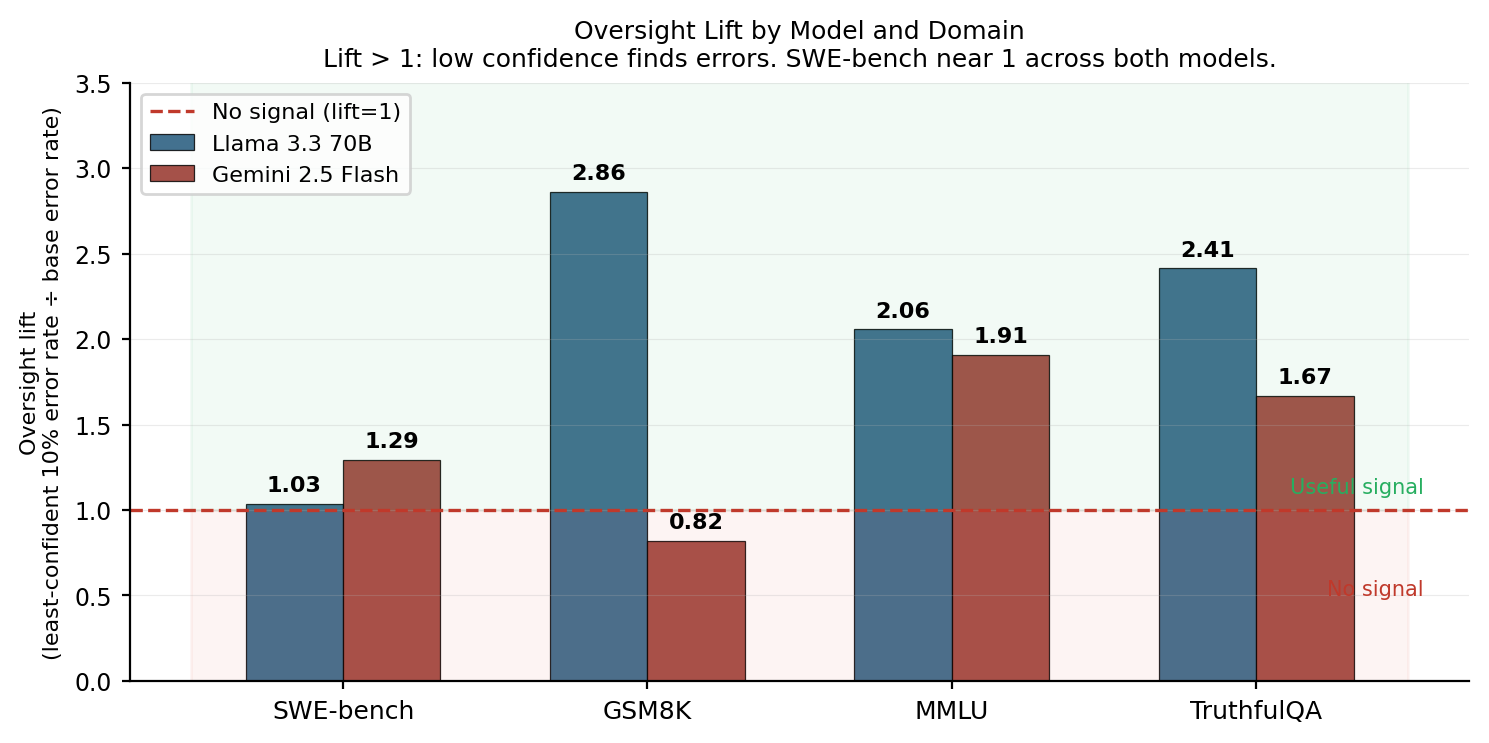
\includegraphics[width=0.95\textwidth]{figures/fig4_lift.png}
\caption{\textbf{Fig.\,1 --- Oversight Lift by Model and Domain.}
Lift = error rate among the least-confident 10\% $\div$ overall base error rate.
Lift~$>1$ (green region): low confidence reliably finds errors; lift~$\approx1$
(red region): the gate adds no value. SWE-bench lift is near~1 for both models
across every configuration tested. GSM8K, MMLU, and TruthfulQA lifts are
1.67--2.86. \textit{This is the paper's primary result: for the two models
evaluated, confidence-gating works on structured QA but not on the SWE-bench
difficulty-judgment task.}}
\label{fig:lift}
\end{figure}

\vspace{6pt}
\begin{figure}[ht]
\centering
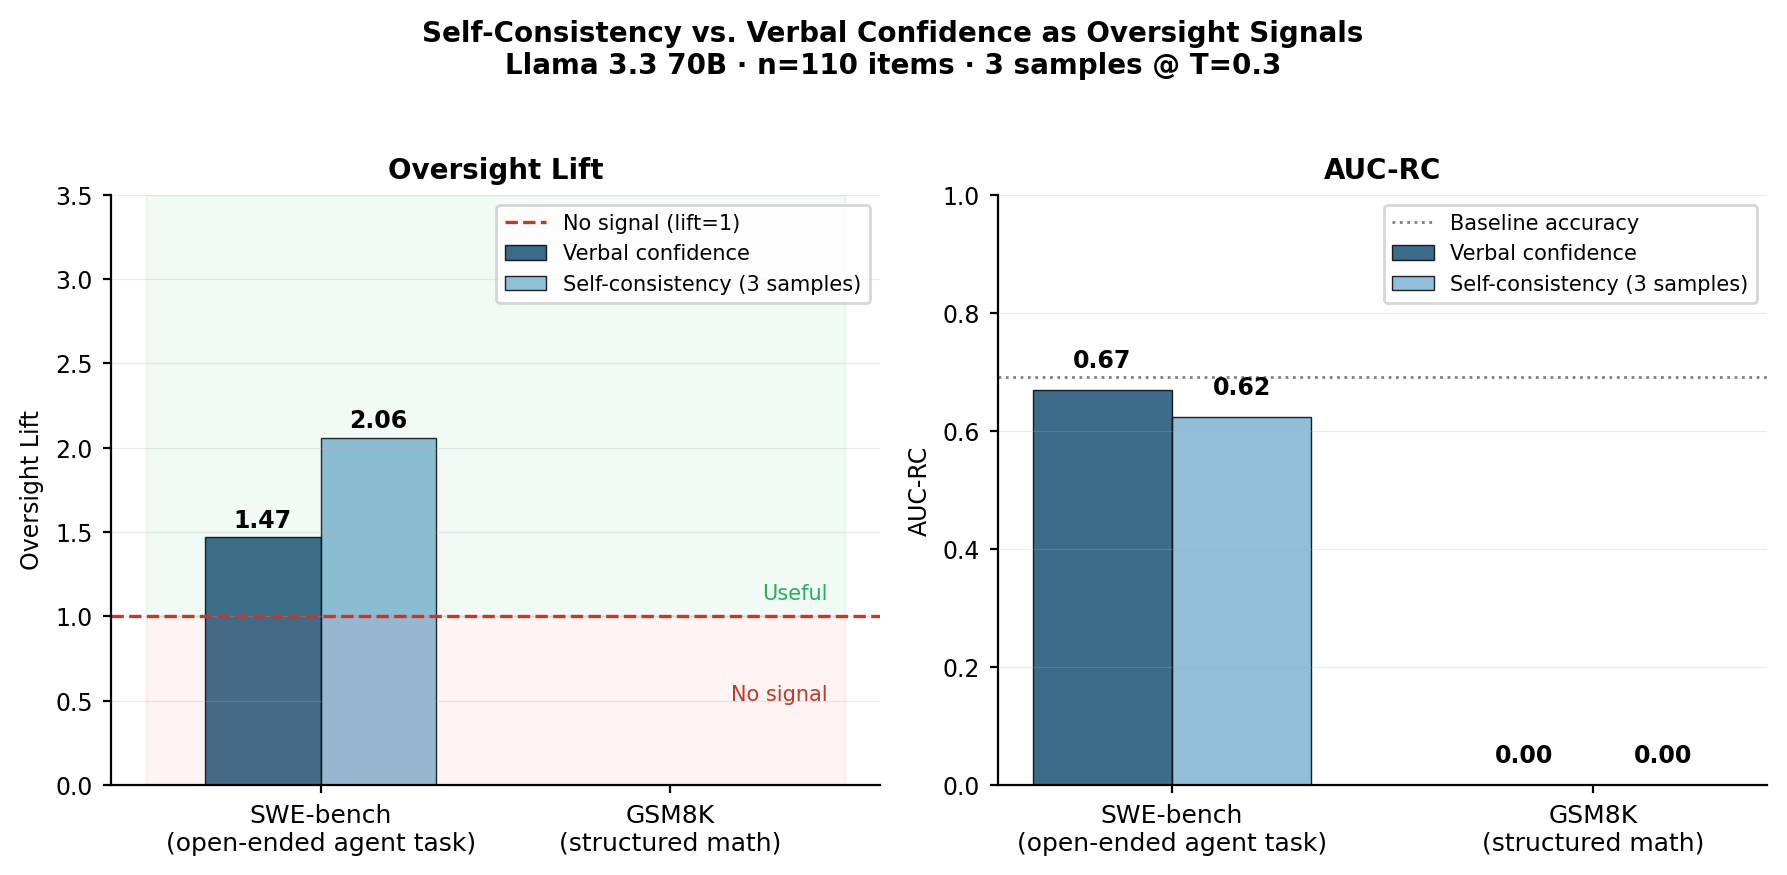
\includegraphics[width=0.80\textwidth]{figures/fig5_sc_comparison.png}
\caption{\textbf{Fig.\,2 --- Self-Consistency vs.\ Verbal Confidence as
Oversight Signals} (Llama~3.3 70B, $n{=}110$). \textit{Left}: oversight lift.
\textit{Right}: AUC-RC. On SWE-bench, self-consistency (3~samples,
$T{=}0.3$) raises lift from~1.47 to~2.06, a 40\% improvement on the task type
where verbal confidence fails. On GSM8K, verbal confidence is the stronger
signal (lift~2.86 vs.\ SC~1.95). Neither method dominates across task types,
suggesting that the choice of uncertainty estimator should be matched to the task.}
\label{fig:sc}
\end{figure}

\vspace{6pt}
\begin{figure}[ht]
\centering
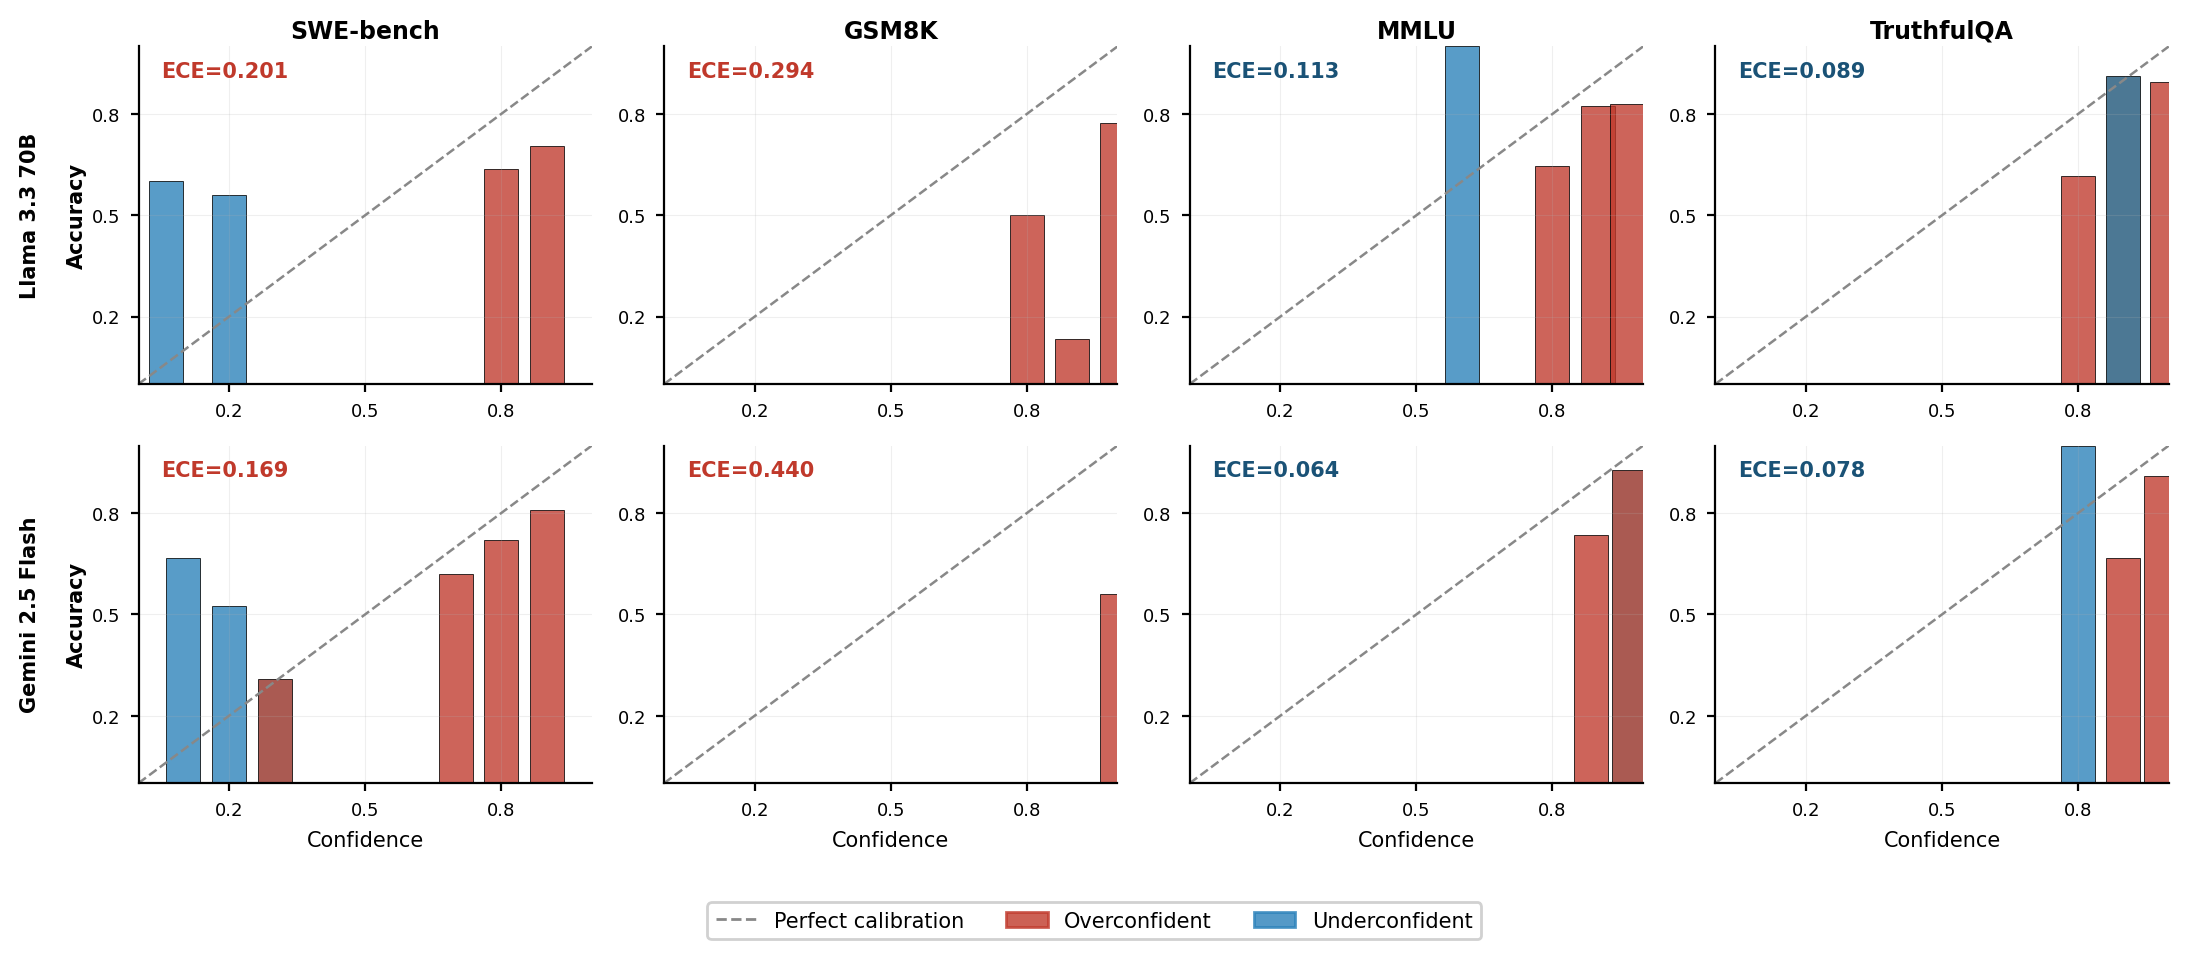
\includegraphics[width=0.95\textwidth]{figures/fig1_reliability.png}
\caption{\textbf{Fig.\,3 --- Reliability Diagrams} (2~models $\times$
4~domains). Bar height is empirical accuracy in each confidence bin; the dashed
diagonal is perfect calibration. Red bars: overconfident (stated confidence
exceeds accuracy). Blue: underconfident. GSM8K panels show systematic
overconfidence for both models, with bars far above the diagonal. On MMLU and
TruthfulQA, calibration is closer to the diagonal but bins are sparse due to
confidence collapse.}
\label{fig:reliability}
\end{figure}

\vspace{6pt}
\begin{figure}[ht]
\centering
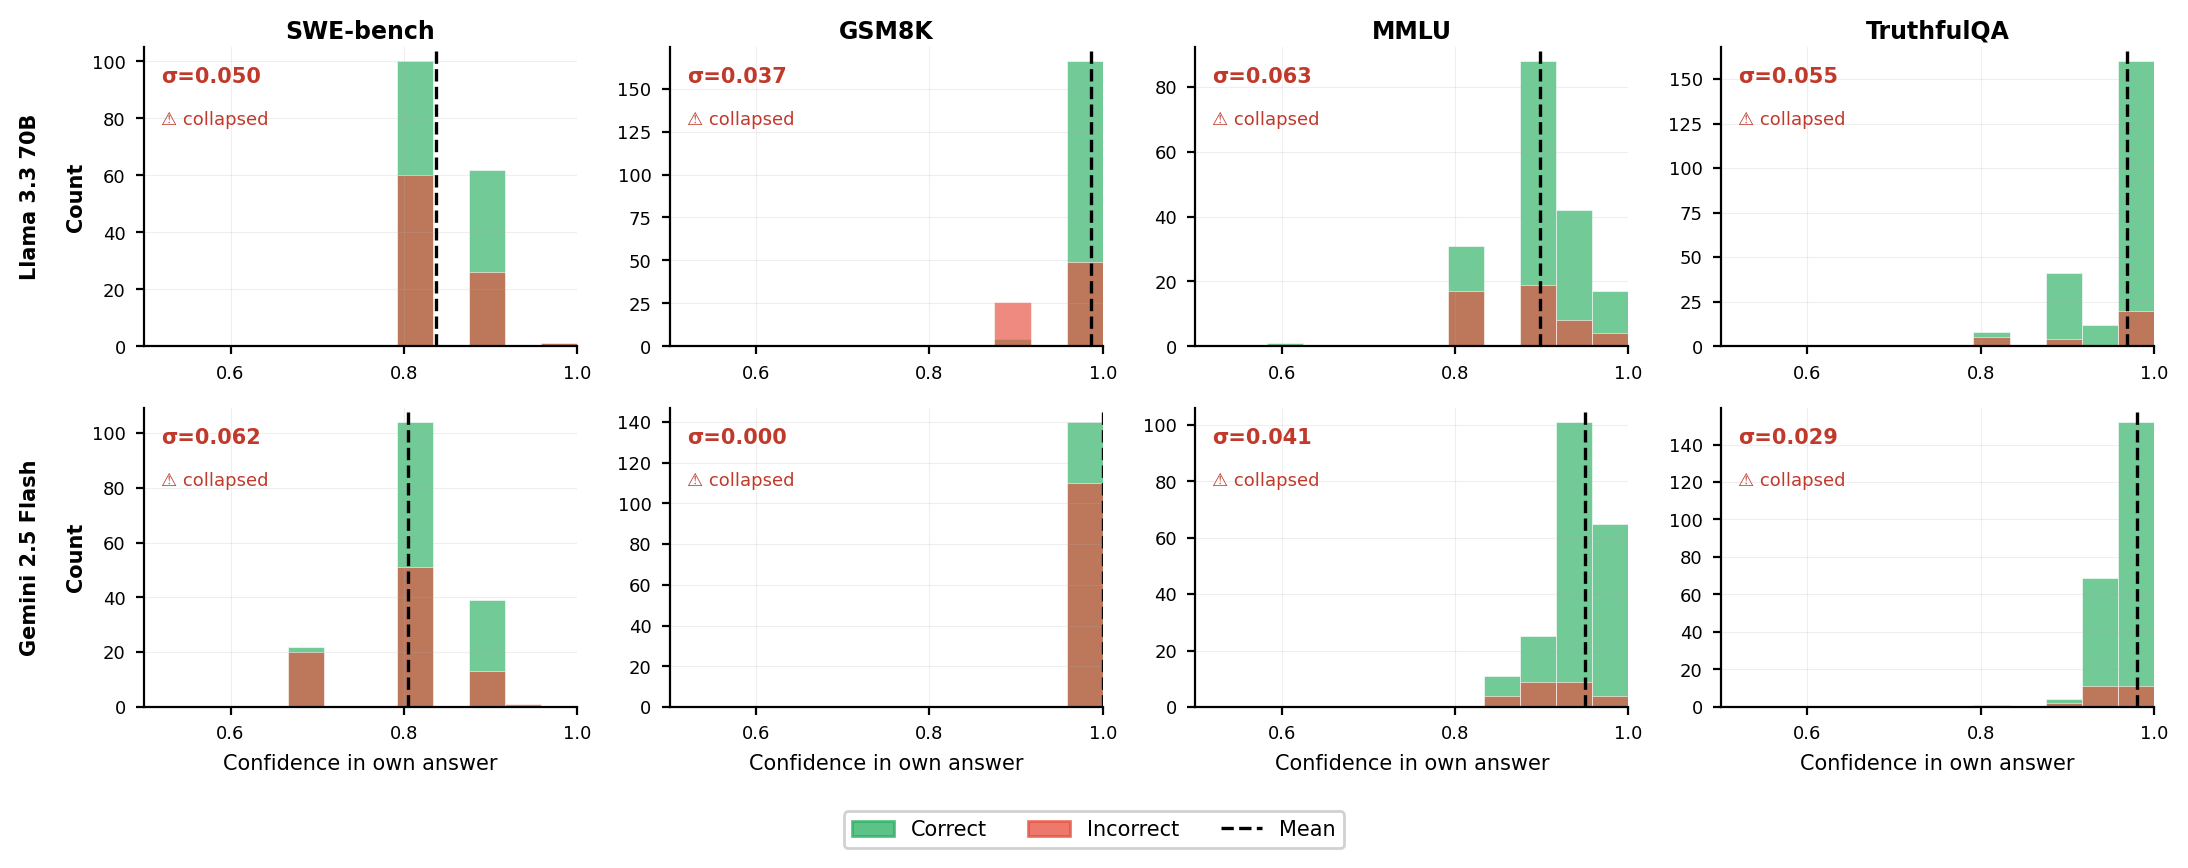
\includegraphics[width=0.95\textwidth]{figures/fig2_confidence.png}
\caption{\textbf{Fig.\,4 --- Confidence Distributions by Domain and Model.}
Histograms split by outcome (green: correct; red: incorrect). Every panel has
$\sigma{<}0.10$ (labelled), indicating confidence collapse: the distributions
of correct and incorrect decisions overlap almost entirely. Gemini's GSM8K
column contains all 250~observations in a single bar at~$1.0$ ($\sigma{=}0.000$).
Because the distributions are indistinguishable, no fixed threshold can
reliably separate reliable from unreliable decisions.}
\label{fig:confidence}
\end{figure}

\vspace{6pt}
\begin{figure}[ht]
\centering
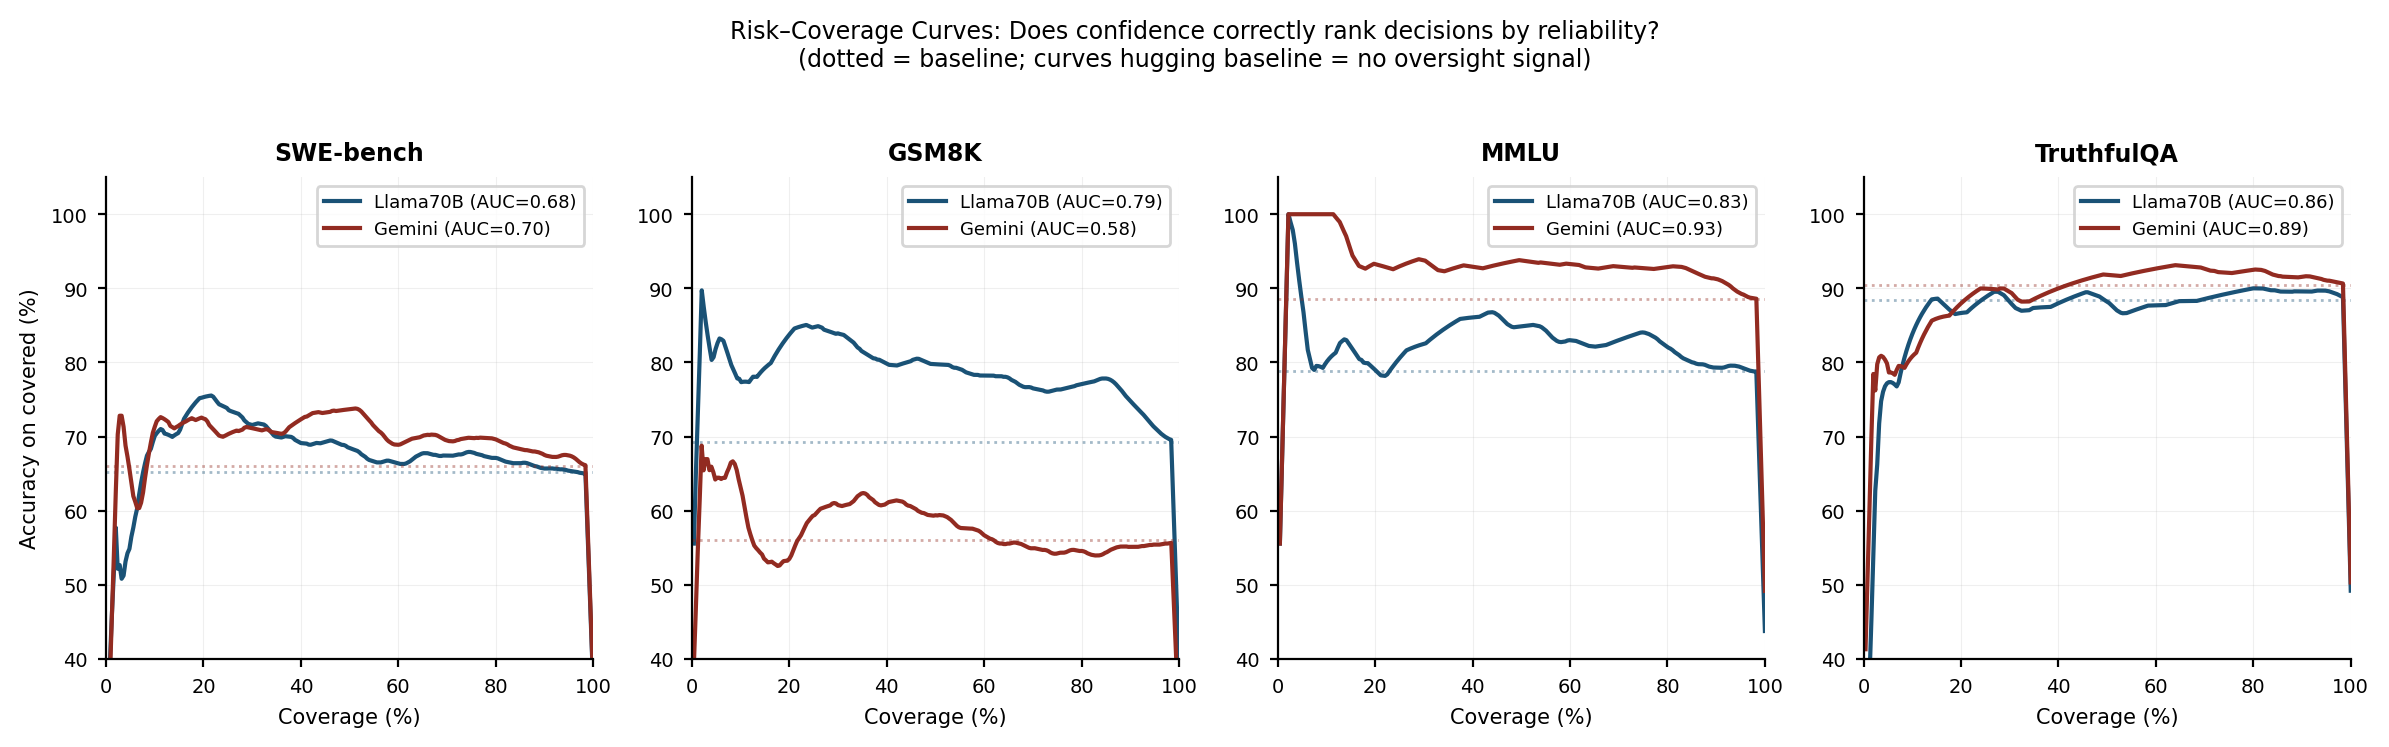
\includegraphics[width=0.95\textwidth]{figures/fig3_riskcoverage.png}
\caption{\textbf{Fig.\,5 --- Risk-Coverage Curves} (one panel per domain).
The $x$-axis is the fraction of decisions handled autonomously (sorted
most-confident first); the $y$-axis is accuracy on that covered set. Dotted
horizontal lines show each model's baseline accuracy. Curves that track the
baseline, as both models do on SWE-bench, indicate that confidence does not
rank decisions by correctness. On GSM8K, MMLU, and TruthfulQA, curves are
meaningfully above baseline at low coverage.}
\label{fig:rc}
\end{figure}

\vspace{6pt}
\begin{figure}[ht]
\centering
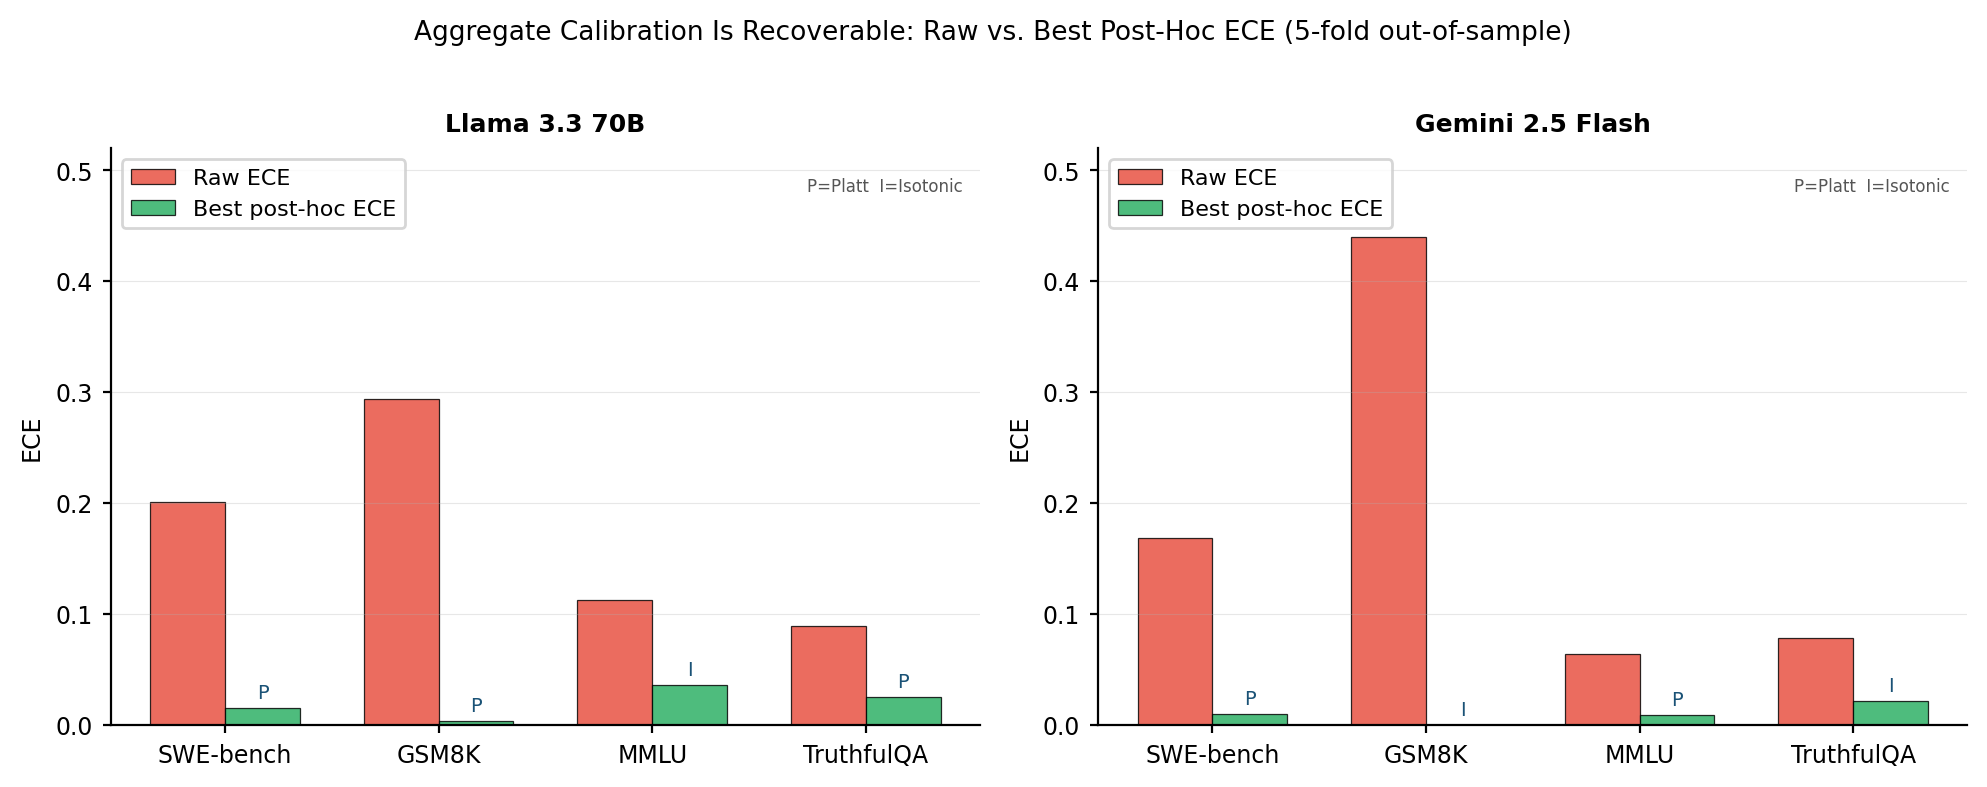
\includegraphics[width=0.86\textwidth]{figures/fig6_calibration.png}
\caption{\textbf{Fig.\,6 --- Aggregate Calibration Before and After Post-Hoc
Correction.} Raw ECE (red) vs.\ best five-fold out-of-sample post-hoc ECE
(green). P$=$Platt scaling, I$=$Isotonic regression. Every condition achieves
$>$50\% relative ECE reduction. \textit{Aggregate calibration is recoverable
without retraining; per-decision discrimination is not.} The Gemini-GSM8K
green bar reaches near-zero because isotonic regression maps the single
confidence value (1.0 for all items) to the mean accuracy---ECE~$=0$ by
construction, not by calibration.}
\label{fig:calibration}
\end{figure}

\end{document}
